\chapter{Introduction\label{sec:intro}}


Our world is a complex compositional system, where simple components are used to create more complex ones and all components interact in a non-trivial way. 
One such component are humans, who have a innate ability to accumulate diverse multi-domain knowledge and learn a rich compositional structure of the surrounding world.
This knowledge allows humans to easily solve a plethora of complex tasks. For example, given a static 2D image of a complex dynamic 3D scene, humans are able to recognize objects, their parts, relationships between them, and predict future events in the scene. Humans can even predict a scene's geographical and demographic context and infer abstract properties such as the sentiment of the scene (\fig{\ref{fig:intro_apps}}, a).
Engineering aims to develop systems and algorithms capable of replacing humans in performing such tasks, especially tasks that are repetitive, laborious or dangerous.
In some practical scenarios such as understanding 2D images, these systems are required to recover the original compositional structure from the input recorded by sensors (\fig{\ref{fig:intro_apps}}, a-c). For example, robots or self-driving cars need to detect objects and their relationships from raw pixels or point clouds. In other scenarios the compositional structure is already provided (\eg by another system or human) and algorithms need to reason about the compositional input to make complex higher-level decisions (\fig{\ref{fig:intro_apps}}, d-f). Example tasks include: predicting properties of molecules, predicting future links between people or predicting properties of biological or artificial neural networks.



\begin{figure}[tbhp]
    \vspace{-10pt}
    \centering
    \small
    \setlength{\tabcolsep}{1pt}
    \begin{tabular}{>{\centering\arraybackslash}p{0.44\textwidth}>{\centering\arraybackslash}p{0.54\textwidth}}
        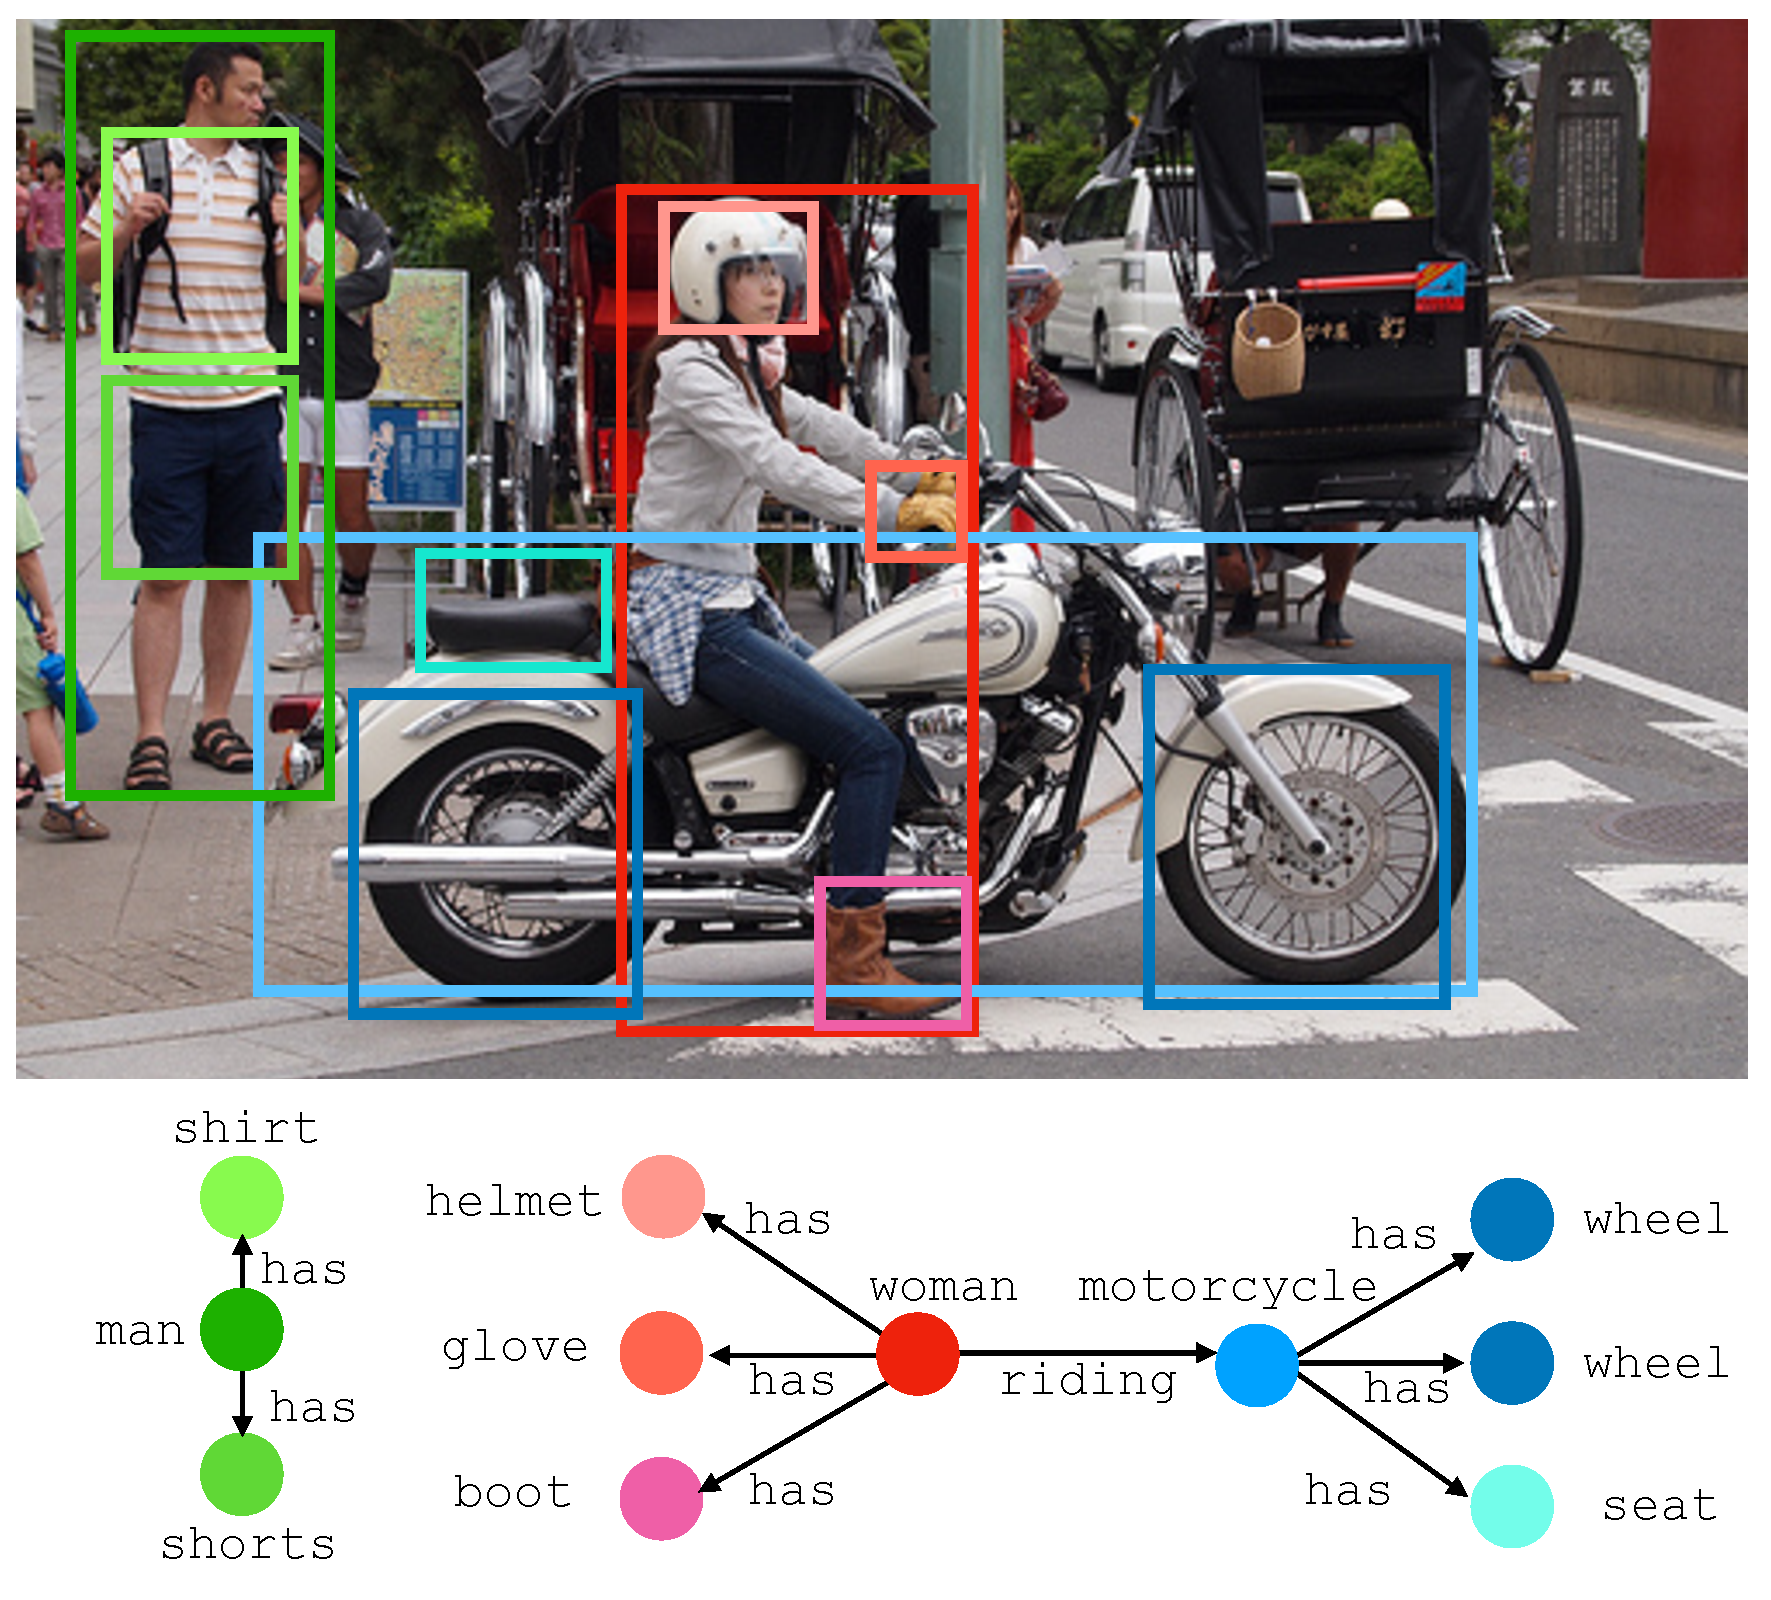
\includegraphics[width=0.3\textwidth, align=c]{Ch1_Intro/motifs_scene_graph.pdf} & {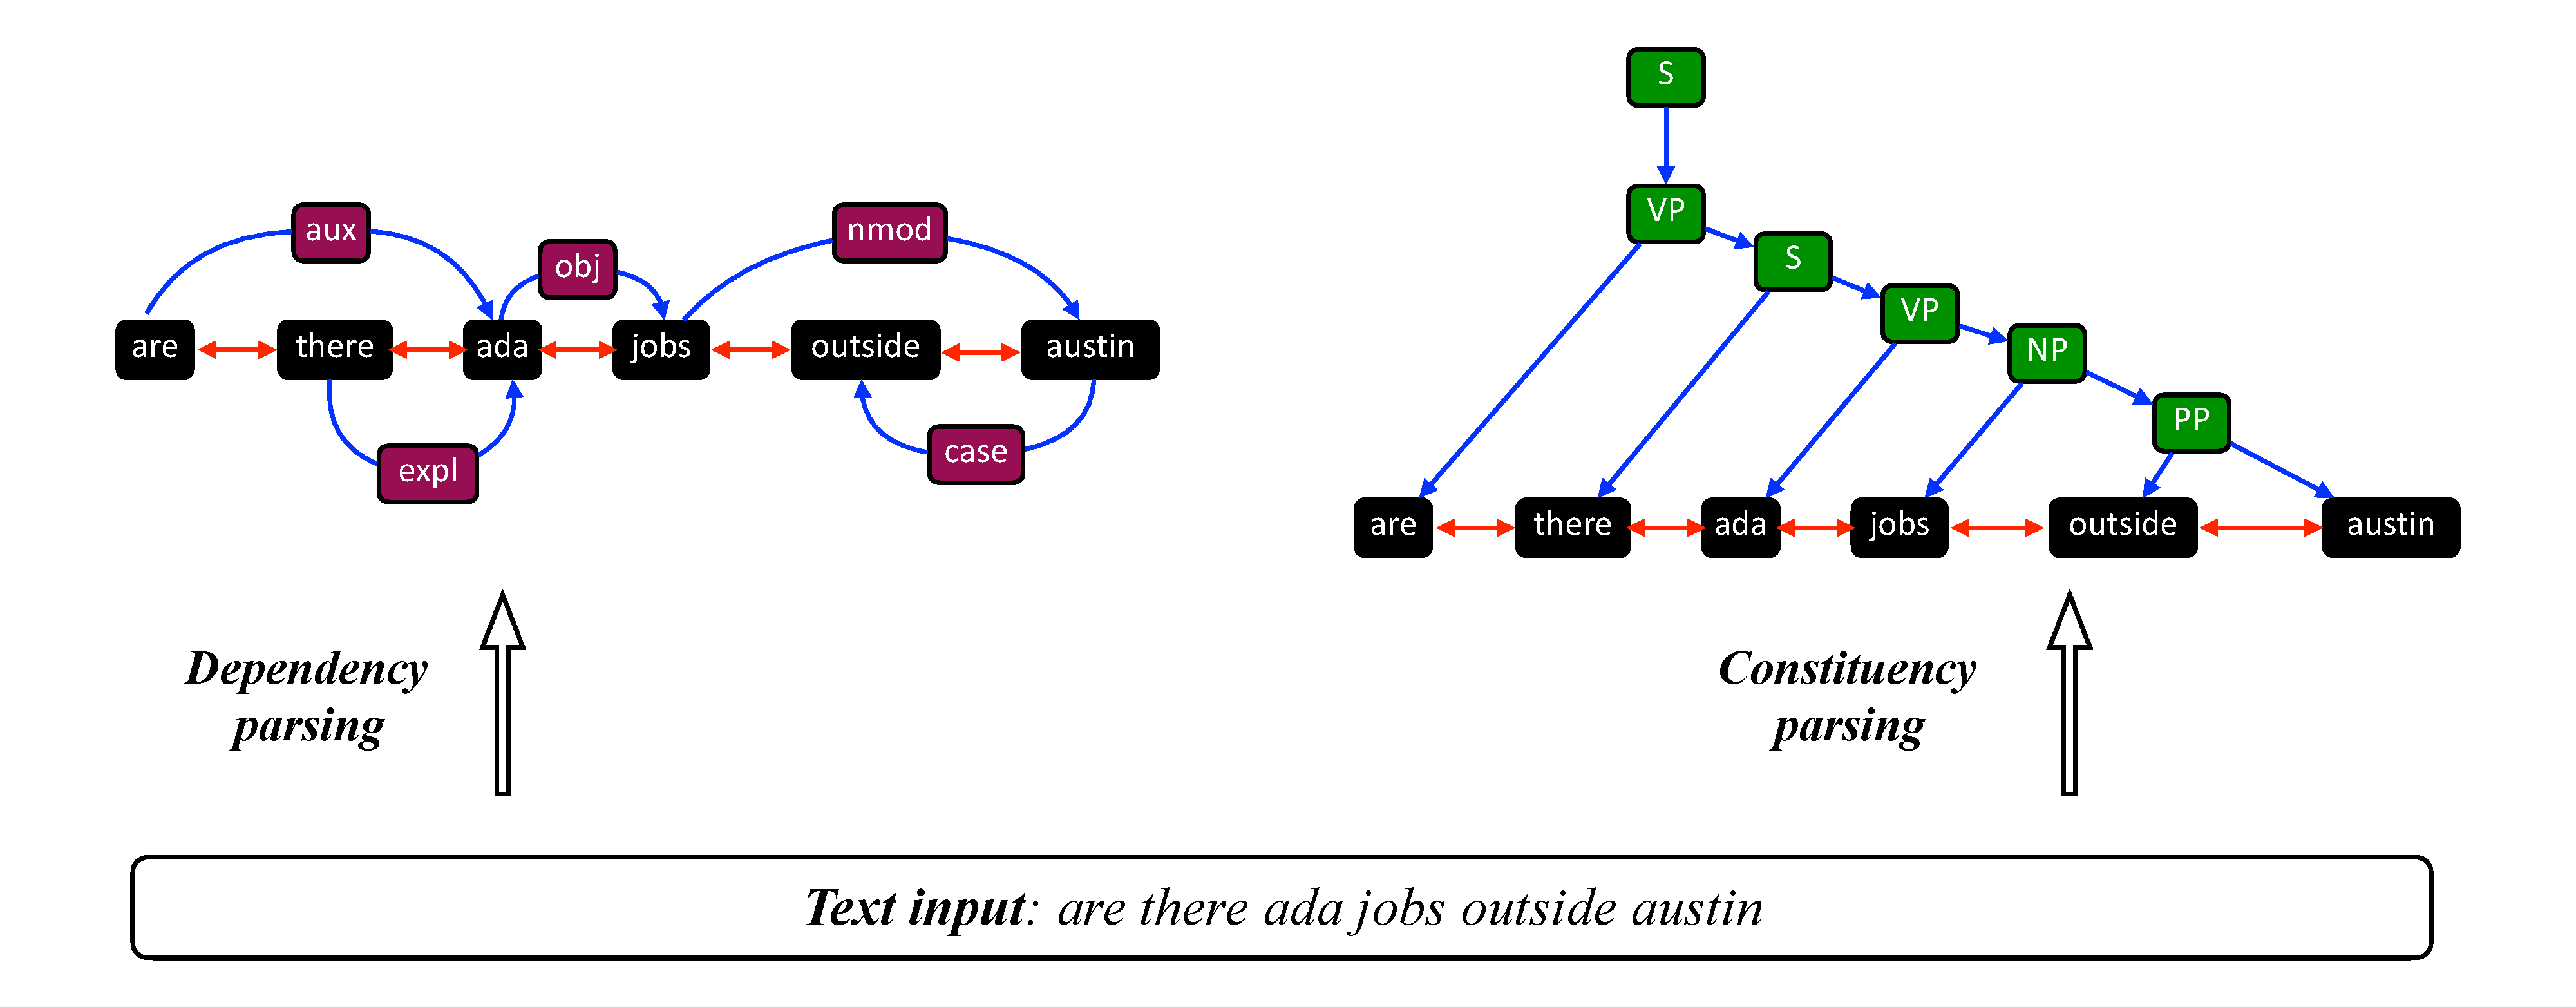
\includegraphics[width=0.53\textwidth, align=c,trim={2cm 12.5cm 36cm 5cm},clip]{Ch1_Intro/graph-construction-v1.pdf}} \\
        (a) Detecting objects and their relationships in a scene~\citep{zellers2018neural} & (b) Modeling language as graphs~\citep{wu2021graph} \\ \\
        
        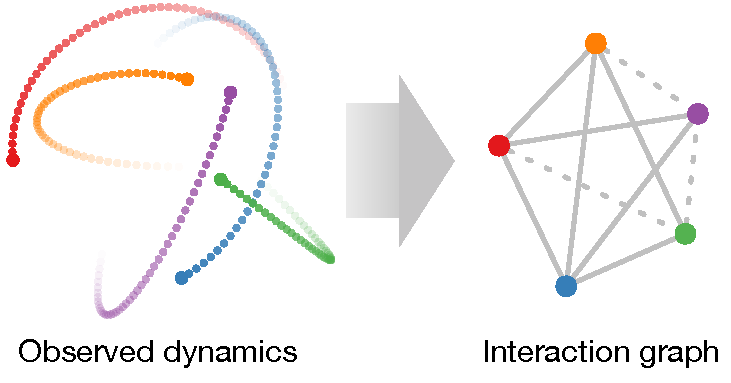
\includegraphics[width=0.35\textwidth, align=c]{Ch1_Intro/nri_physics_graph.pdf} & 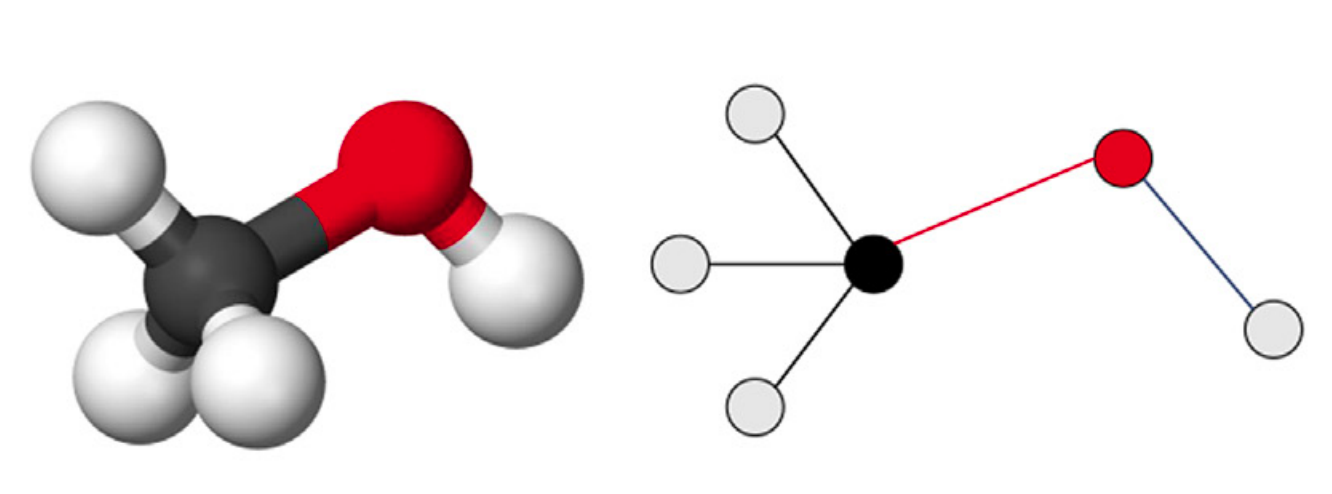
\includegraphics[width=0.5\textwidth, align=c]{Ch1_Intro/molecule_graph.png} \\
        (c) Inferring interactions in physical systems~\citep{kipf2018neural} & (d) Analyzing molecules~\citep{zhou2020graph} \\ \\
        
        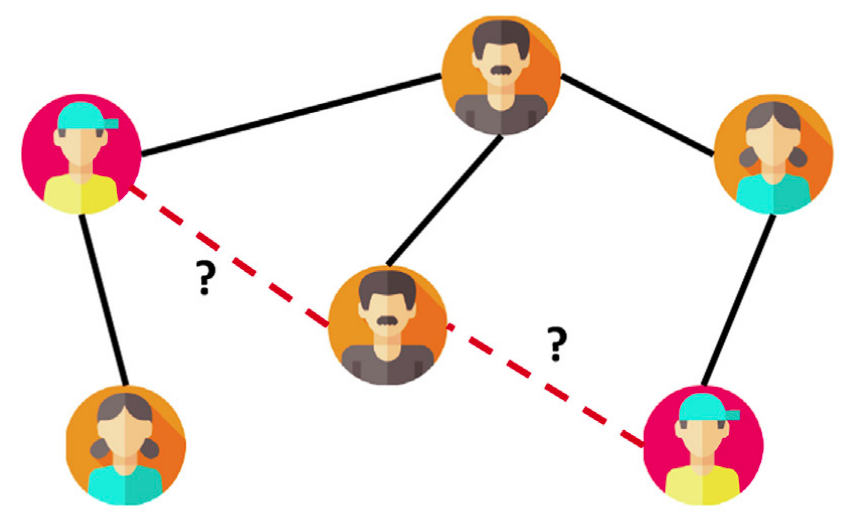
\includegraphics[width=0.3\textwidth, align=c]{Ch1_Intro/fig1_c2.png} & 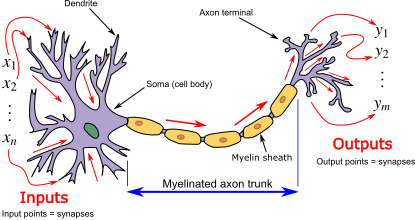
\includegraphics[width=0.3\textwidth, align=c]{Ch1_Intro/Neuron3.png} 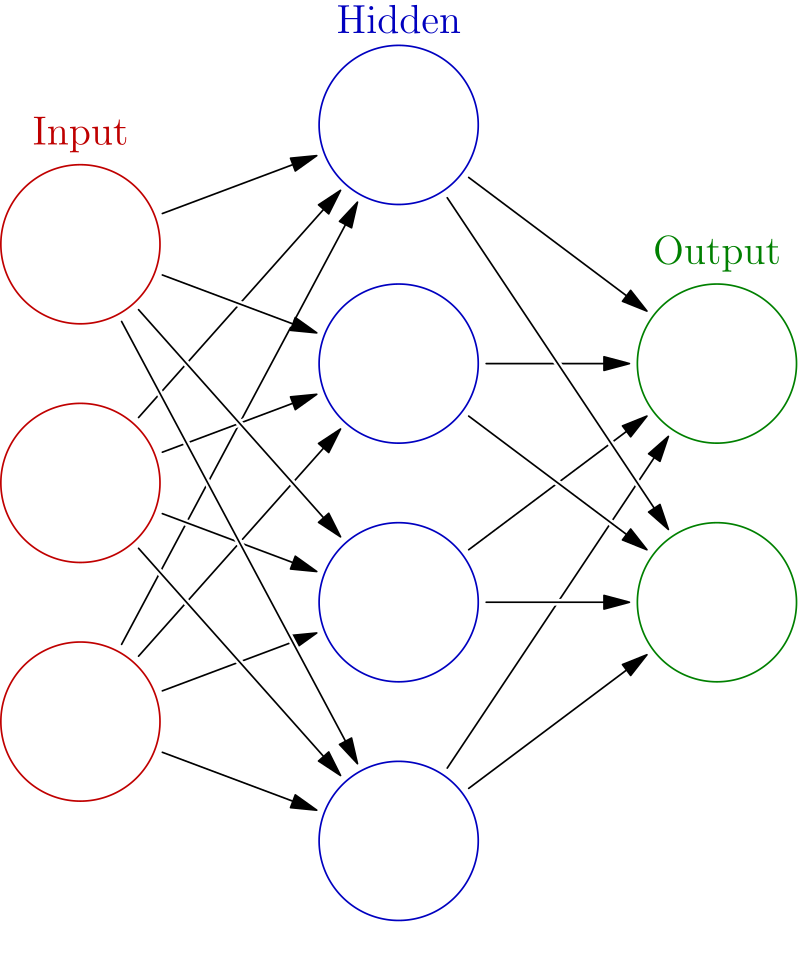
\includegraphics[width=0.17\textwidth, align=c]{Ch1_Intro/Colored_neural_network.png} \\
        (e) Predicting links in social networks~\citep{zhou2020graph} & (f) Predicting properties of neural networks\textsuperscript{1} \\
        
    \end{tabular}
    \caption{\small Example applications of graph reasoning methods. \textsuperscript{1}Images are obtained from {\footnotesize \url{https://en.wikipedia.org/wiki/Artificial_neural_network}} and {\footnotesize \url{https://en.wikipedia.org/wiki/Biological_neuron_model}}.}
    \label{fig:intro_apps}
    %\vspace{-10pt}
\end{figure}




To develop algorithms able of inferring a compositional structure from raw sensory data or algorithms predicting structure's properties, we first need to define a data abstraction suitable for this kind of tasks.
In mathematics and computer science there exists a convenient abstraction specifically introduced to model compositional and relational structures. This abstraction is called a graph, in which nodes correspond to the components of the structure and edges correspond to interactions between the components.
For example, molecules are often represented as graphs with nodes corresponding to atoms or more complex elements and edges corresponding to chemical bonds (Fig.~\ref{fig:intro_apps}, d). Similarly, social networks are graphs with nodes being people and edges being different kinds of relationships between them (Fig.~\ref{fig:intro_apps}, e). Likewise, a biological or artificial neural network is a graph wherein nodes can be neurons and edges can be connections between them (Fig.~\ref{fig:intro_apps}, f). 
Having modeled data as graphs, algorithms tackling the associated tasks need to be developed.


Tasks illustrated in \fig{\ref{fig:intro_apps}} can be approached by manually designing task-specific rules or algorithms. However, recently there has been a spike in performance on such tasks using deep learning methods. In particular, deep neural networks (DNNs) require less human interventions and instead learn task-specific rules and algorithms from data and experience. DNNs currently dominate across visual, language and graph tasks~\citep{lecun2015deep}. Specifically, state-of-the-art convolutional neural networks (CNNs)~\citep{krizhevsky2012imagenet,he2016deep} reach or even outperform~\citep{he2015delving,cai2019onceforall} humans in tasks such as large-scale image classification, \eg ImageNet~\citep{russakovsky2015imagenet}. In the graph domain, many tasks have been successfully solved by DNNs operating on graphs, called Graph Neural Networks (\gnns)~\citep{gori2005new, scarselli2008graph, bronstein2017geometric,zhou2020graph}. 
DNNs continue to improve and extend their scope, becoming an essential part of real world applications~\citep{brown2020language}.

\begin{figure}[tbhp]
    \centering
    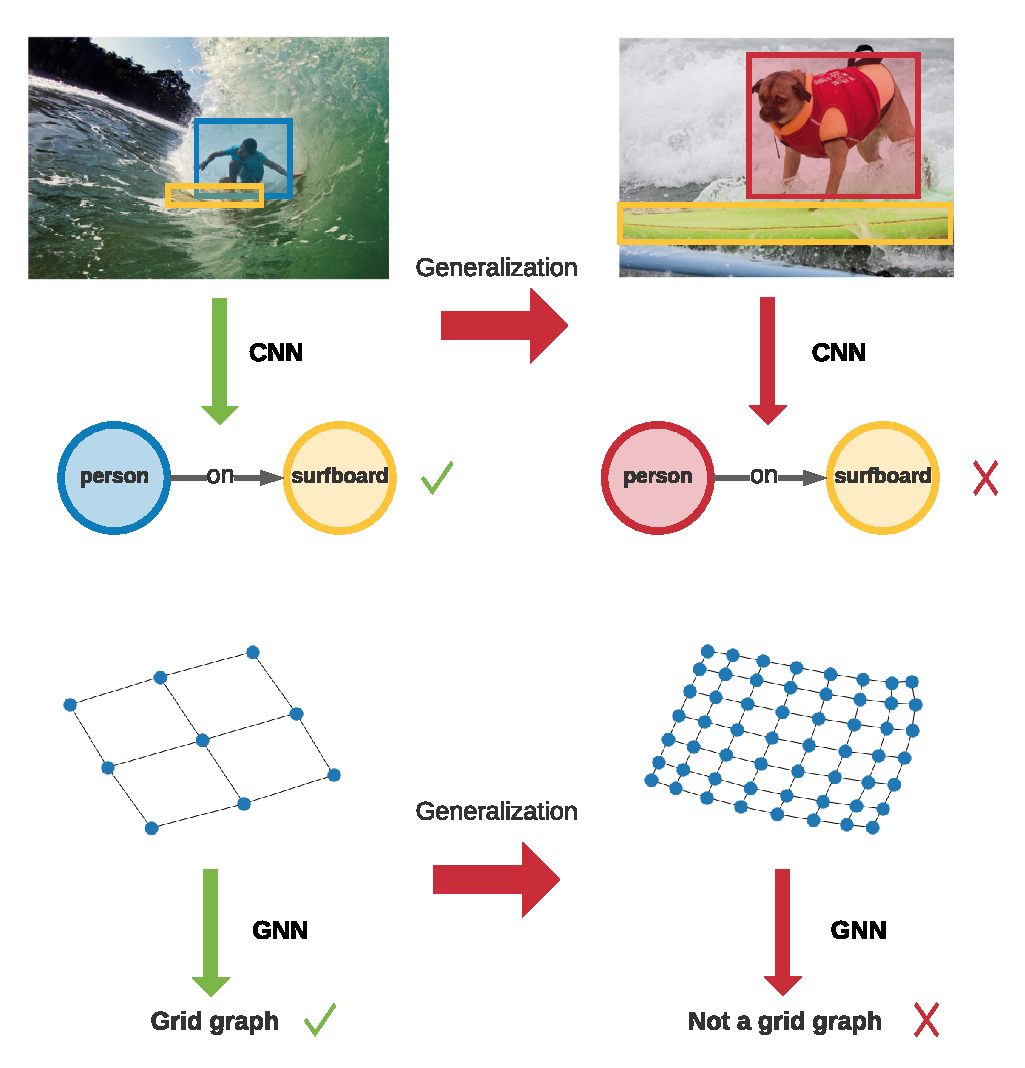
\includegraphics[width=0.6\textwidth, align=c]{Ch1_Intro/intro_generalization.pdf}
    \vspace{-10pt}
    \caption{\small Machine learning methods for images, graphs and other domains can accurately reason about the \IID samples (left). However, reasoning on test samples that are somewhat different from or correspond to the tail of the training distribution (right) remains challenging. In the graph example (bottom), both the small and large graph represent so called grid (mesh or lattice) graphs. }
    \label{fig:intro_generalization}
\end{figure}

Despite the extreme success of DNNs, they have certain limitations and this thesis mainly addresses the two of them. The first challenge is fundamental and concerns the decrease of DNNs' performance when they observe somewhat unusual inputs~\citep{hendrycks2019benchmarking,galloway2019batch,szegedy2013intriguing}. For example in the image domain, the dog on a surfboard can be confused with a person, since in the data used to train CNNs persons appear more frequently on surfboards than dogs (\fig{\ref{fig:intro_generalization}}, top). In the graph domain, a GNN trained to reason about smaller graphs, can fail to accurately reason about larger graphs~\citep{yehudai2021local} (\fig{\ref{fig:intro_generalization}}, bottom).
While there is still limited understanding what exactly makes CNNs or GNNs fail in such cases, a high-level explanation is that learning-based methods make an assumption that all training and test samples are independently and identically distributed (\IID)~\citep{shen2021towards}. In practice (as illustrated in \fig{\ref{fig:intro_generalization}}), this assumption is often violated, leading to inaccurate predictions or poor generalization. 
%In machine learning terms, such DNNs are not robust or do not generalize well to distribution shifts. 
Such behavior is often unacceptable in critical applications such as self-driving cars or health care, where errors can be fatal.
To highlight this issue and develop a more rigorous understanding of DNNs' generalization properties, a variety of research frameworks have been proposed~\citep{lust2020survey,shen2021towards,hendrycks2019benchmarking,hupkes2019compositionality,garg2020generalization}. Despite these efforts, in many tasks the progress remains slow. For instance, in the scene graph generation task state-of-the-art CNNs show a $\sim$10 fold decrease in performance on test images containing unusual or unseen visual compositions~\citep{tang2020unbiased,knyazev2020graph,suhail2021energy}. In this thesis, we develop empirical frameworks to study generalization failure in CNNs and GNNs, leading to improvements in the visual and graph domains respectively.\looseness-1

The second limitation of DNNs pertains to the challenge of extending their scope to more problems where manually-designed algorithms still dominate. Before the rise of DNNs, researchers and practitioners focused tremendous efforts on designing features to better solve a concrete task, \eg image classification~\citep{lowe2004distinctive}. The advent of deep learning showed that in many settings features learned by DNNs outperformed features designed by humans~\citep{krizhevsky2012imagenet}. This encouraged researchers and practitioners to extend the scope of DNNs in many directions. One notable direction has been the design of stronger DNN architectures\footnote{Generally speaking, a DNN architecture is defined by the types of neural network layers, their number and connectivity between them.} to better solve a given task. Similar to pre-deep learning feature design, architecture design has been recently overtaken by neural architecture search methods that \emph{learn} a DNN architecture, replacing and outperforming human-designed DNN architectures~\citep{zoph2016neural,liu2018darts,ren2020comprehensive}.
Yet many aspects of DNN practice still require much human engineering effort. 


In particular, optimization algorithms used to train DNNs are still manually-designed.
For example, one of the dominant algorithms is stochastic gradient descent (SGD). SGD is a manually-designed algorithm based on computing gradients \wrt a highly \textit{non-convex} loss function and the gradient-based rules to update DNN parameters according to \textit{convex} optimization theory~\citep{jain2017non}. Replacing optimization algorithms such as SGD with DNN counterparts may reveal more optimal update rules~\citep{andrychowicz2016learning}. Learnable optimizers remain one of the oldest directions that still have only limited success~\citep{schmidhubermetalearning,metz2020tasks}.
Yet, by analogy with other successful directions, if DNNs could replace SGD, then dramatic advances might follow. In this thesis, we make a step towards that long-standing and ambitious goal. Specifically, we develop graph reasoning methods that allow us to predict performant parameters of DNNs represented as graphs. Following the focus of previous chapters on aspects of generalization, we take into consideration samples beyond \IID when developing and evaluating parameter prediction methods. This extends the scope of this thesis to more practical and challenging scenarios.\looseness-1
